\documentclass{article}
\usepackage{geometry}
\usepackage{subcaption}
\usepackage{parskip}
\usepackage{graphicx}
\usepackage{pythonhighlight}
\newcommand{\code}[1]{\texttt{#1}}

\geometry{
  a4paper,
  margin=1in
}

\title{NLarge your dataset: Data Augmentation for NLP}

\author{
  Ng Tze Kean \\
  \texttt{ngtzekean@gmail.com}
  \and
  Dexter Gui \\
  \texttt{dexter@email.com}
}

\begin{document}

\maketitle

\begin{abstract}

  In this report, we explore the application of data augmentation techniques for
  Natural Language Processing (NLP) using a variety of methods including Large
  Language Models (LLMs). We demonstrate the effectiveness of these techniques in
  enhancing the diversity and robustness of the training data, potentially
  improving the performance of NLP models. We present our methodology,
  experimental results, and discuss the implications of our findings.

  Overall, we found that use of statistical methods such as substitution for data
  augmentation has limited applications. The use of more advanced deep learning
  models such as RNN with attention mechanisms tend to perform better in this
  task. The best results were obtained using Large Language Models (LLMs) for
  data augmentation, which significantly improved the performance of the model.

\end{abstract}

\section{Introduction}

Data augmentation is a widely used technique in machine learning to enhance the
diversity and robustness of training datasets. By artificially expanding the
dataset, data augmentation helps improve the generalization capabilities of
models, particularly in scenarios where labeled data is scarce or expensive to
obtain. In the context of Natural Language Processing (NLP), data augmentation
poses unique challenges due to the complexity and variability of human
language.

Traditional data augmentation methods in NLP, such as synonym replacement,
random insertion, and back-translation, have shown limited effectiveness in
generating diverse and meaningful variations of text data. These methods often
fail to capture the nuanced semantics and contextual dependencies inherent in
natural language, leading to suboptimal improvements in model performance.

Recent advancements in deep learning, particularly the development of Large
Language Models (LLMs) like GPT-2, GPT-3, and T5, have opened new avenues for
data augmentation in NLP. These models, pre-trained on vast corpora of text
data, possess a remarkable ability to generate coherent and contextually
relevant text. Leveraging LLMs for data augmentation involves generating
synthetic data samples by providing prompts based on existing training
examples.

In this report, we explore the application of LLMs for data augmentation in
NLP. We investigate the effectiveness of using LLMs to generate diverse and
high-quality augmented data, and assess the impact of this approach on the
performance of NLP models. Our study includes a detailed examination of the
methodology, experimental results, and a discussion of the implications of our
findings. Through this exploration, we aim to provide insights into the
potential benefits and challenges of using LLMs for data augmentation in NLP.

\subsection{Training and Evaluation}
% Training process, evaluation metrics

To evaluate the performance gain of the data augmentation techniques, we
augmented the dataset at different levels: 5\%, 10\%, and 20\%. We then trained
the same Recurrent Neural Network (RNN) model to perform sentiment
classification on the validation dataset and noted the gains in performance.

\subsubsection{Model Architecture for Sentiment Classification}

The RNN model architecture consists of an embedding layer, followed by an RNN
layer, and a fully connected layer with a sigmoid activation function for
binary classification. The model was trained using the Adam optimizer with a
learning rate of \code{5e-4} and binary cross-entropy loss.

We adopted a pre-trained word embedding model to initialize the embedding layer
to transfer knowledge from the pre-trained model to our sentiment classification
task. The RNN layer uses a simple hidden layer our target is to train that task
layer to perform sentiment classification.


Our primary measure of improvement is the accuracy gain on the validation
dataset by the task specific RNN model. We also monitor the loss curves to
ensure that the model is not overfitting to the training data. Our hypothesis
is that the model will generalize better to unseen data with the augmented
dataset through various means to increase the volume of the corpus in meaningful
manners that will help the model learn and overfit less to the training data.

For each level of augmentation (5\%, 10\%, and 20\%), we monitored the training
and validation accuracy of the model to assess the impact of data augmentation
on model performance.

\subsection{Data Augmentation using Random Substitution}

In this subsection, we analyze the performance of data augmentation using
random substitution. Random substitution is a traditional data augmentation
technique where words in the text are randomly replaced with their synonyms.
This method aims to introduce variability into the dataset, potentially
improving the robustness and generalization capabilities of NLP models.

To evaluate the effectiveness of random substitution, we conducted experiments
with different levels of augmentation: 5\%, 10\%, and 20\% of the dataset. The
performance of the models trained with these augmented datasets was assessed
using standard evaluation metrics.

\subsubsection{Results and Analysis}
Our results indicate that data augmentation at 5\% of the dataset performs best
compared to the 10\% and 20\% augmentation levels. Specifically, the model
trained with 5\% augmented data achieved the highest accuracy and lowest loss,
as illustrated in Figure \ref{fig:random_substitution_loss}. The performance
metrics for the 10\% and 20\% augmentation levels showed a decline, suggesting
that excessive random substitution may introduce noise and reduce the quality
of the training data.

% insert image 
\begin{figure}[ht]
  \centering
  \begin{subfigure}[b]{0.3\textwidth}
    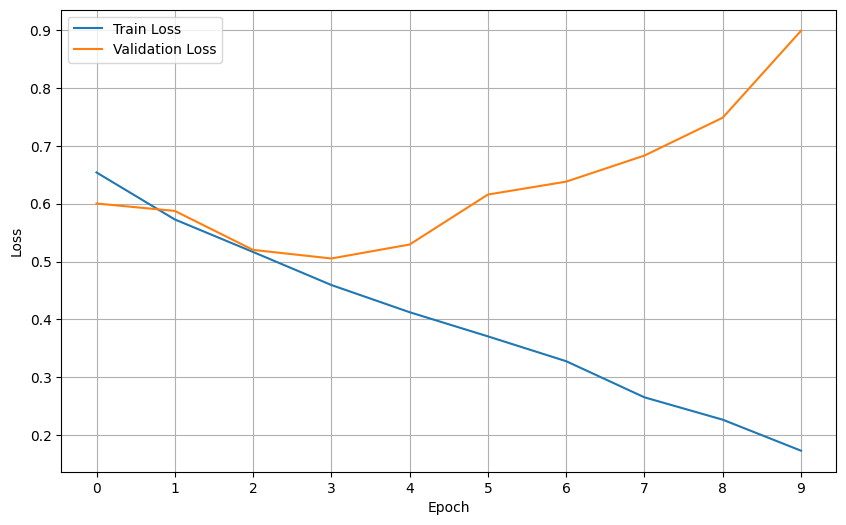
\includegraphics[width=\textwidth]{img/random_5.png}
    \caption{5\% Augmentation}
    \label{fig:random_5}
  \end{subfigure}
  \hfill
  \begin{subfigure}[b]{0.3\textwidth}
    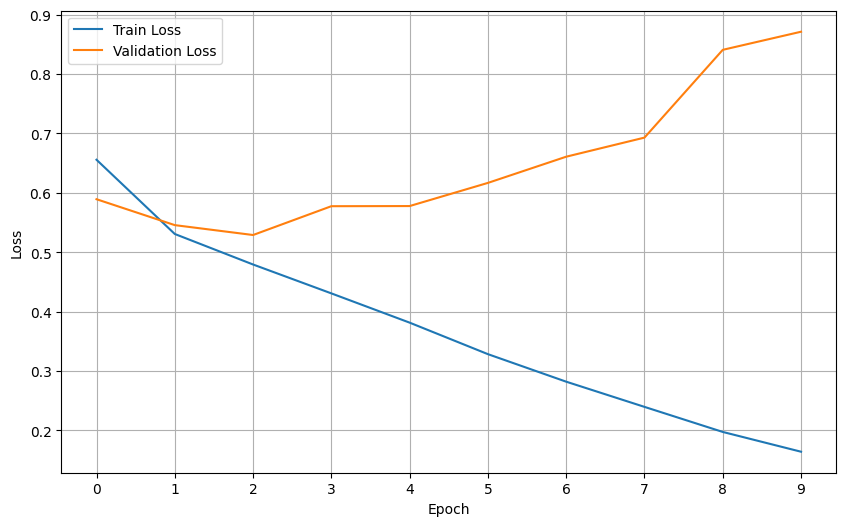
\includegraphics[width=\textwidth]{img/random_10.png}
    \caption{10\% Augmentation}
    \label{fig:random_10}
  \end{subfigure}
  \hfill
  \begin{subfigure}[b]{0.3\textwidth}
    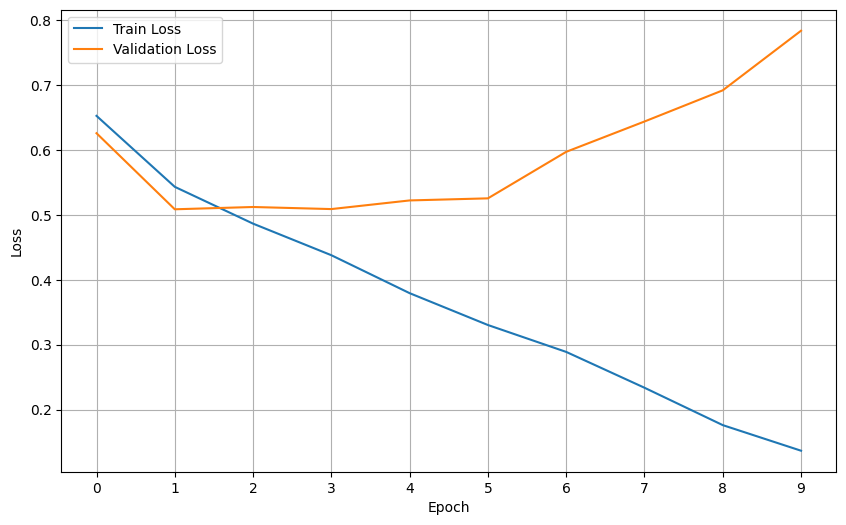
\includegraphics[width=\textwidth]{img/random_20.png}
    \caption{20\% Augmentation}
    \label{fig:random_20}
  \end{subfigure}
  \caption{Loss graphs for random substitution data augmentation at 5\%, 10\%, and 20\% levels.}
  \label{fig:random_substitution_loss}
\end{figure}

The superior performance at the 5\% augmentation level can be attributed to the
balance between introducing variability and maintaining the integrity of the
original data. At higher augmentation levels, the increased randomness may lead
to less meaningful and contextually relevant substitutions, thereby diminishing
the overall quality of the augmented dataset.

In conclusion, our analysis demonstrates that while random substitution can be
a useful data augmentation technique, it is crucial to carefully select the
augmentation level to avoid degrading the dataset quality. The 5\% augmentation
level strikes an optimal balance, enhancing the model's performance without
introducing excessive noise.

\subsection{Data Augmentation using Synonym Substitution}

\subsubsection{Results and Analysis}

% insert image 
\begin{figure}[ht]
  \centering
  \begin{subfigure}[b]{0.3\textwidth}
    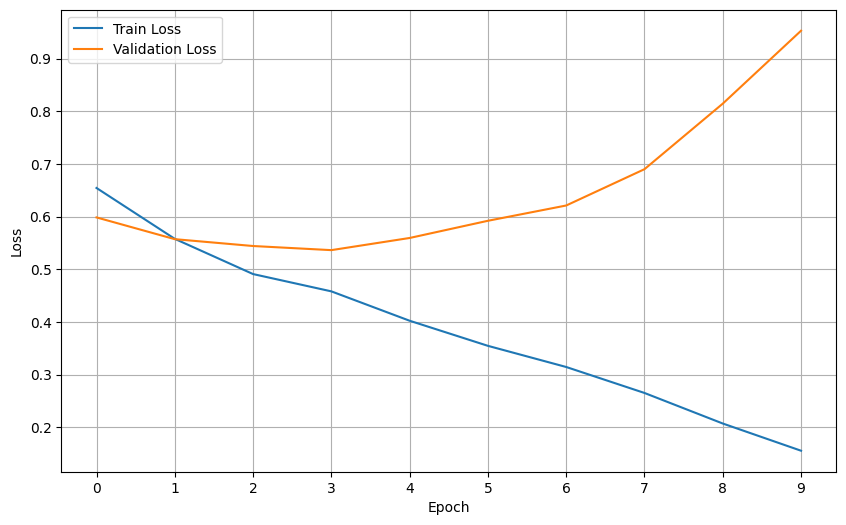
\includegraphics[width=\textwidth]{img/synonym_loss_5.png}
    \caption{5\% Augmentation}
    \label{fig:synonym_loss_5}
  \end{subfigure}
  \hfill
  \begin{subfigure}[b]{0.3\textwidth}
    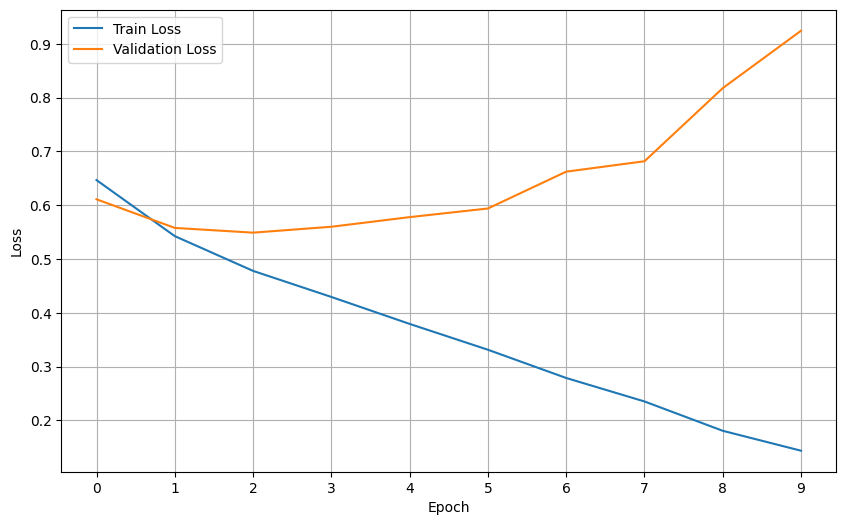
\includegraphics[width=\textwidth]{img/synonym_loss_10.png}
    \caption{10\% Augmentation}
    \label{fig:synonym_loss_10}
  \end{subfigure}
  \hfill
  \begin{subfigure}[b]{0.3\textwidth}
    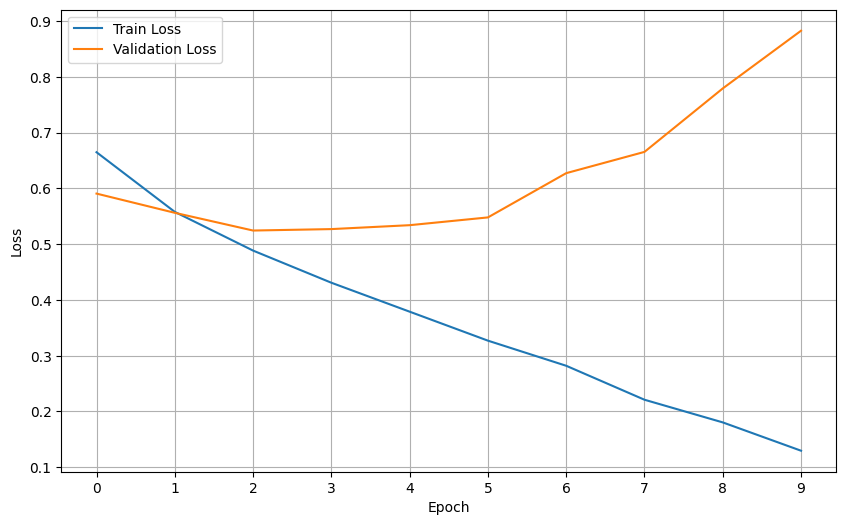
\includegraphics[width=\textwidth]{img/synonym_loss_20.png}
    \caption{20\% Augmentation}
    \label{fig:synonym_loss_20}
  \end{subfigure}
  \caption{Loss graphs for synonym substitution data augmentation at 5\%, 10\%, and 20\% levels.}
  \label{fig:synonym_substitution_loss}
\end{figure}

\subsection{Data Augmentation using LLMs}

To enhance the diversity and robustness of our dataset, we employed a data
augmentation technique leveraging pre-trained Large Language Models (LLM) from
the Transformers library.

Specifically, we utilized the model to generate synthetic data samples by
providing prompts based on existing training examples. By carefully controlling
the generation parameters, we were able to produce high-quality, diverse, and
relevant augmented samples that expanded the scope of our training data,
potentially improving model generalization and performance.

\subsubsection{LLM selection}

We would like to note some of the challenges of selection of the LLM model for
data augmentation. The choice of the model is crucial as it determines the
quality of the generated samples. We experimented with several models,
including GPT-2, GPT-3, and T5. As we tried to perform prompt engineering to
generate diverse samples, we found that these models could not adequately
paraphrase the training data, more often than not, producing the exact same
text or slightly modified versions of the original text.

We suspect that these LLM do not perform well due to the lack of contextual
information in the prompt. We hypothesize that the models require more
contextual information to generate diverse samples. We realised that a model
that allows us to specify a role for the prompt, we would be able to generate
more diverse samples.

\subsubsection{Prompt Engineering}

We proceeded to experiment with the Qwen model, with some of the techniques
applied from \cite{promptingguide}. We found that the Qwen model allows us to
specify a role for the prompt, which allows us to instruct the model to
specifically only paraphrase the verbs and structure of the sentence. This
allows us to generate a text that differs from the original text, while still
retaining the meaning of the original text.

\subsubsection{Results and Analysis}

We observed that with the Qwen model, we were able to generate diverse and
relevant samples, yet the performance of the model did not improve and in fact
there was significant degradation in the performance of the model. This can
be seen from Figure \ref{fig:llm_substitution_loss} and Table \ref{table:rnn_performance}.
This is very
unexpected as we hypothesized that the diverse samples would improve the
performance of the model. Our hypothesis that using a expert model to increase
the diversity of the samples would improve the performance of the model was
not supported by the results.


\begin{figure}[ht]
  \centering
  \begin{subfigure}[b]{0.3\textwidth}
    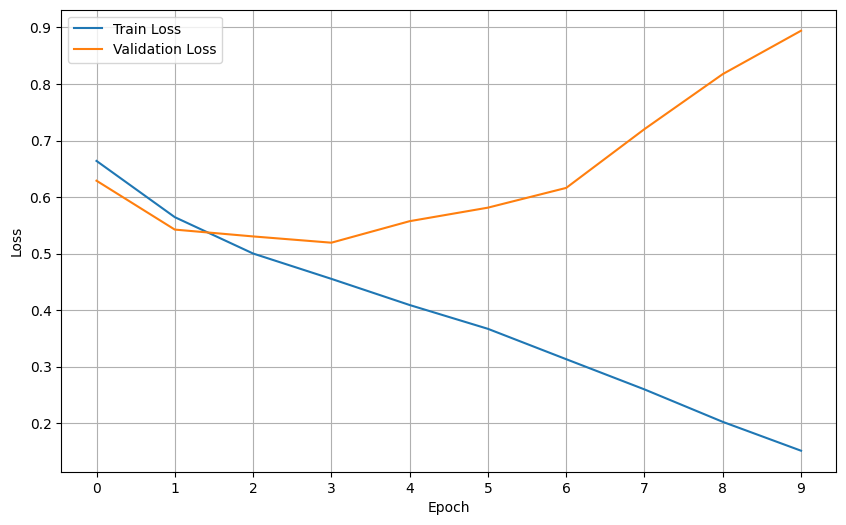
\includegraphics[width=\textwidth]{img/llm_loss_5.png}
    \caption{5\% Augmentation}
    \label{fig:llm_loss_5}
  \end{subfigure}
  \hfill
  \begin{subfigure}[b]{0.3\textwidth}
    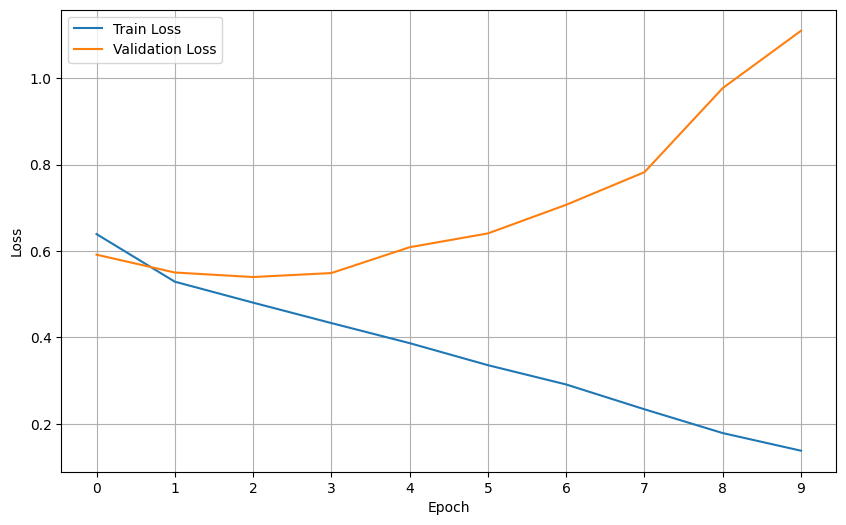
\includegraphics[width=\textwidth]{img/llm_loss_10.png}
    \caption{10\% Augmentation}
    \label{fig:llm_loss_10}
  \end{subfigure}
  \hfill
  \begin{subfigure}[b]{0.3\textwidth}
    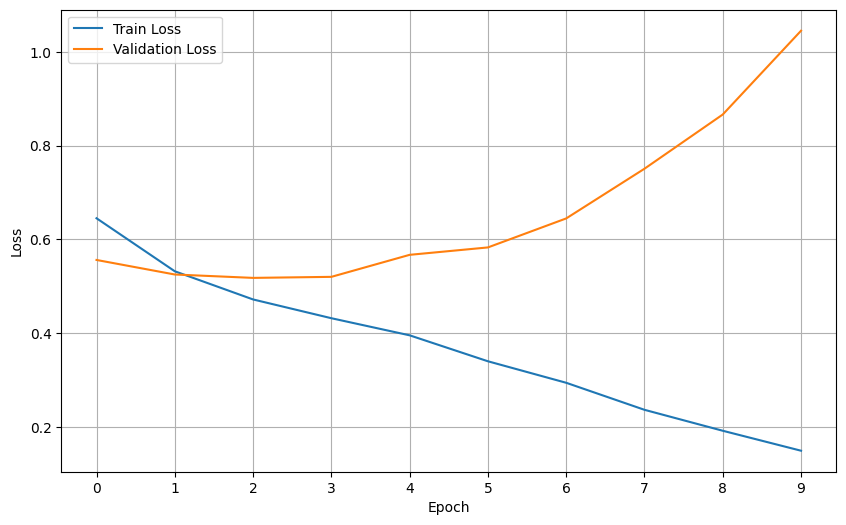
\includegraphics[width=\textwidth]{img/llm_loss_20.png}
    \caption{20\% Augmentation}
    \label{fig:llm_loss_20}
  \end{subfigure}
  \caption{Loss graphs for llm substitution data augmentation at 5\%, 10\%, and 20\% levels.}
  \label{fig:llm_substitution_loss}
\end{figure}

We examined the possible causes of this unexpected result and found that the
augmentation generated by the Qwen model was too long that the RNN suffered
from vanishing gradients. We hypothesize that there was 2 main issues.
% bullet points with numbers
\begin{enumerate}
  \item Vanishing gradients due to the long sequences generated
  \item RNN suffering from the long sequences generated
\end{enumerate}

\begin{table}[ht]
  \centering
  \begin{tabular}{|c|c|c|}
    \hline
    \textbf{Augmentation Level} & \textbf{Train Accuracy} & \textbf{Validation Accuracy} \\
    \hline
    5\% &  0.947 & 0.717 \\
    \hline
    10\% & 0.950 & 0.697 \\
    \hline
    20\% & 0.945 & 0.695 \\
    \hline
  \end{tabular}
  \caption{Performance of RNN model with different levels of data augmentation with 100 token per sample limit.}
  \label{table:rnn_performance}
\end{table}

We tailored our approach in 2 ways: we limited the token length of the generated
samples to 20 tokens and we changed the RNN model to a Long Short-Term Memory
(LSTM) model to better handle the long sequences. We found that the performance
of the model improved significantly, and the model was able to learn and
generalize better.


\section{Discussion}

We find it interesting that the use of statistical methods such as synonym


\section{Conclusion}
% Summarize your findings and future work

\bibliographystyle{plain}
\bibliography{bibliography.bib}

\end{document}